\PassOptionsToPackage{dvipsnames,svgnames,x11names}{xcolor}
\documentclass[tikz,border=8pt]{standalone}
\usetikzlibrary{arrows.meta,positioning,calc,shapes,shadows,decorations.pathmorphing,shapes.geometric,backgrounds,decorations.markings,decorations.pathreplacing,decorations.text,fit,shapes.misc,shapes.arrows,matrix,bending,3d,chains,intersections,shapes.symbols,svg.path,shapes.multipart,snakes,shapes.callouts,angles,quotes}
\providecolor{gold}{RGB}{212,175,55}
\providecolor{silver}{RGB}{192,192,192}
\providecolor{bronze}{RGB}{205,127,50}
\providecolor{darkblue}{RGB}{0,0,139}
\providecolor{lightblue}{RGB}{173,216,230}
\providecolor{darkgreen}{RGB}{0,100,0}
\providecolor{lightgreen}{RGB}{144,238,144}
\providecolor{darkred}{RGB}{139,0,0}
\providecolor{navy}{RGB}{0,0,128}
\providecolor{skyblue}{RGB}{135,206,235}
\providecolor{beige}{RGB}{245,245,220}
\providecolor{cream}{RGB}{255,253,208}
\usepackage{amsmath}
\usepackage{amssymb}
\usepackage{fontawesome5}
\usetikzlibrary{fadings,shadows.blur,patterns,patterns.meta}

\definecolor{srccolor}{RGB}{33, 150, 243}
\definecolor{vpcolor}{RGB}{244, 67, 54}
\definecolor{mathcolor}{RGB}{103, 58, 183}

\begin{document}
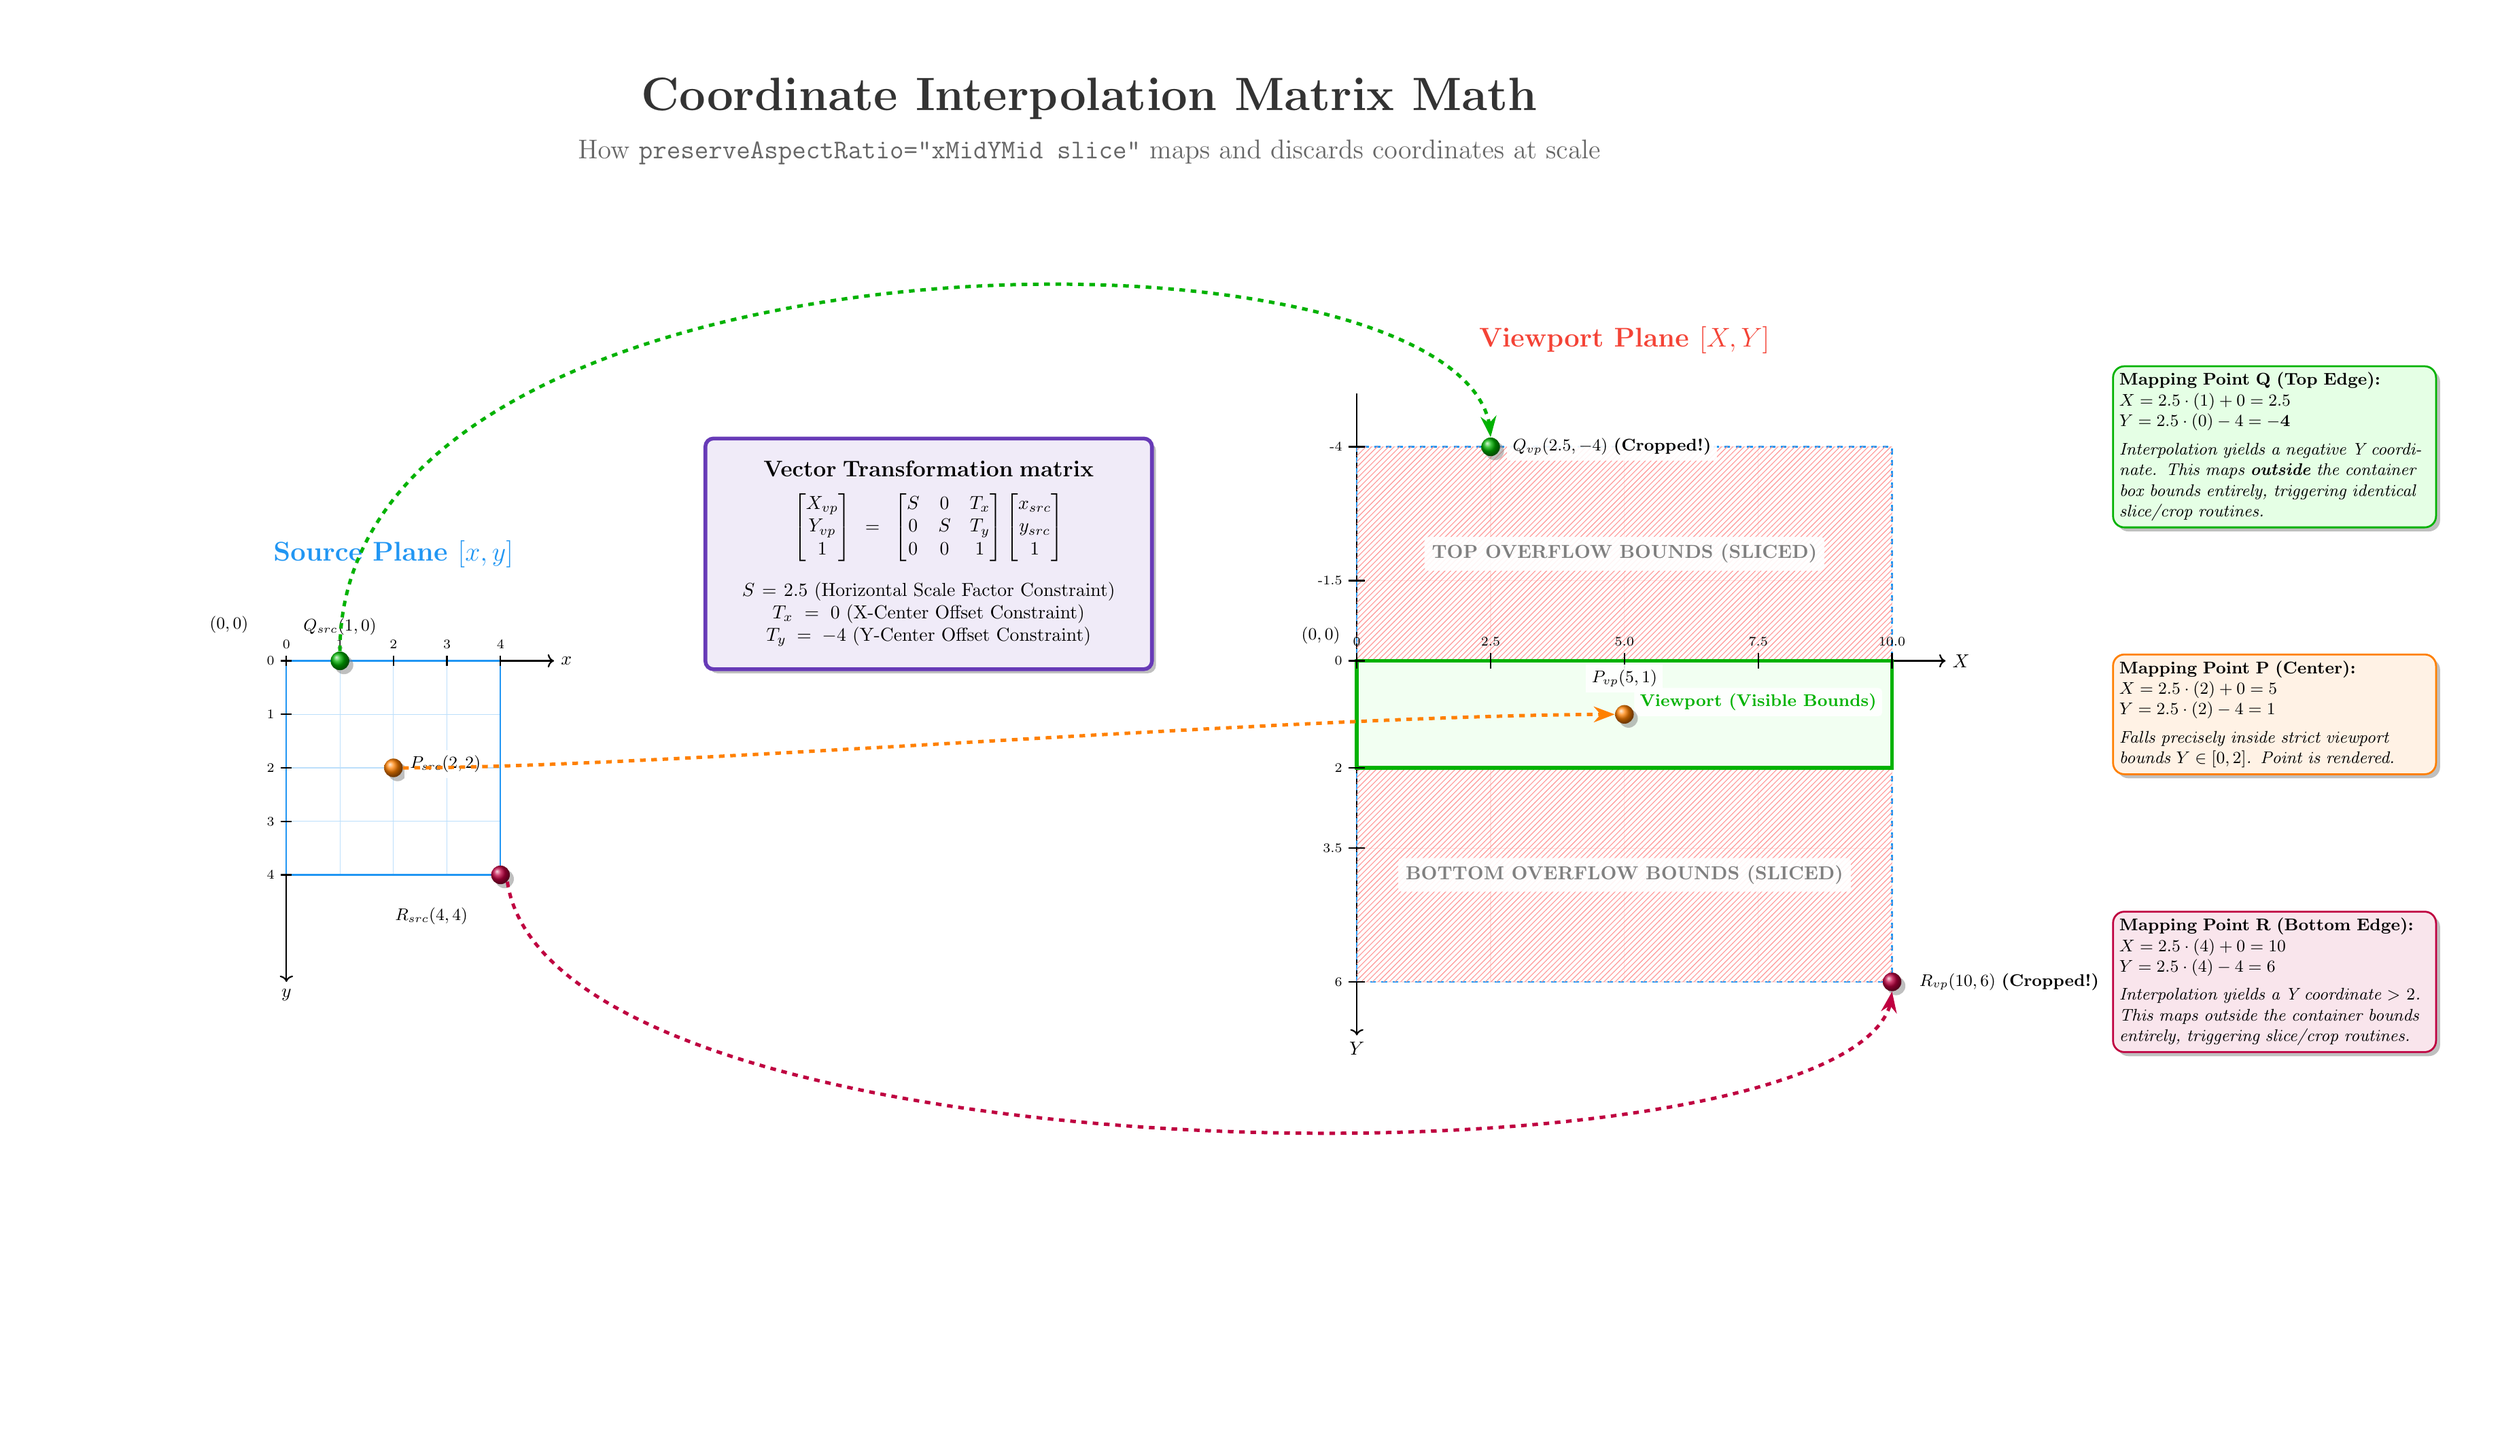
\begin{tikzpicture}
% --- 0. BACKGROUND CANVAS ---
\fill[white] (-20, -8) rectangle (26, 18);

% --- 1. HEADER COMPONENTS ---
\node[font=\Huge\bfseries, text=black!80] at (0, 16.5) {Coordinate Interpolation Matrix Math};
\node[font=\Large, text=black!60] at (0, 15.5) {How \texttt{preserveAspectRatio="xMidYMid slice"} maps and discards coordinates at scale};

% --- 2. SOURCE PLANE (LEFT) ---
\node[font=\Large\bfseries, text=srccolor] at (-13, 8) {Source Plane $[x, y]$};

% Axes (CSS coords: origin top-left, Y descends)
\draw[->, thick] (-15, 6) -- (-10, 6) node[right] {$x$};
\draw[->, thick] (-15, 6) -- (-15, 0) node[below] {$y$};
\node[anchor=south east, font=\small, fill=white, fill opacity=0.9, text opacity=1, inner sep=3pt] at (-15.6, 6.4) {$(0,0)$};

% Intrinsic Grid (step=1)
\draw[srccolor!30, step=1] (-15, 2) grid (-11, 6);
\draw[thick, srccolor] (-15, 2) rectangle (-11, 6);

% Source Axis Ticks (Every 1 unit)
\foreach \x/\val in {-15/0, -14/1, -13/2, -12/3, -11/4} {
    \draw[thick] (\x, 6.1) -- (\x, 5.9);
    \node[above, font=\scriptsize] at (\x, 6.1) {\val};
}
\foreach \y/\val in {6/0, 5/1, 4/2, 3/3, 2/4} {
    \draw[thick] (-15.1, \y) -- (-14.9, \y);
    \node[left, font=\scriptsize] at (-15.1, \y) {\val};
}

% 3D Sphere Points in Source Plane
\node[circle, ball color=green!70!black, drop shadow, inner sep=3.5pt] (Qsrc) at (-14, 6) {};
\node[fill=white, fill opacity=0.9, text opacity=1, inner sep=2pt, font=\small, anchor=south] at (-14, 6.4) {$Q_{src} (1, 0)$};

\node[circle, ball color=orange, drop shadow, inner sep=3.5pt] (Psrc) at (-13, 4) {};
\node[fill=white, fill opacity=0.9, text opacity=1, inner sep=3pt, font=\small, anchor=south west] at (-12.8, 3.8) {$P_{src} (2, 2)$};

\node[circle, ball color=purple, drop shadow, inner sep=3.5pt] (Rsrc) at (-11, 2) {};
\node[fill=white, fill opacity=0.9, text opacity=1, inner sep=3pt, font=\small, anchor=north east] at (-11.5, 1.5) {$R_{src} (4, 4)$};

% --- 3. TRANSFORMATION MATRIX (CENTER) ---
\node[fill=mathcolor!10, draw=mathcolor, line width=2pt, rounded corners=1ex, inner sep=12pt, text width=7.5cm, align=center, drop shadow] at (-3, 8) {
    \textbf{\large Vector Transformation matrix} \\[8pt]
    $\begin{bmatrix} X_{vp} \\ Y_{vp} \\ 1 \end{bmatrix} = \begin{bmatrix} S & 0 & T_x \\ 0 & S & T_y \\ 0 & 0 & 1 \end{bmatrix} \begin{bmatrix} x_{src} \\ y_{src} \\ 1 \end{bmatrix}$ \\[10pt]
    $S = 2.5$ (Horizontal Scale Factor Constraint) \\
    $T_x = 0$ (X-Center Offset Constraint) \\
    $T_y = -4$ (Y-Center Offset Constraint)
};

% --- 4. TARGET PLANE (RIGHT) ---
\node[font=\Large\bfseries, text=vpcolor] at (10, 12) {Viewport Plane $[X, Y]$};

% Axes
\draw[->, thick] (5, 6) -- (16, 6) node[right] {$X$};
\draw[->, thick] (5, 11) -- (5, -1) node[below] {$Y$};
\node[anchor=south east, font=\small, fill=white, fill opacity=0.9, text opacity=1, inner sep=3pt] at (4.8, 6.2) {$(0,0)$};

% Scaled Space Grid (step=2.5)
\draw[vpcolor!15, step=2.5] (5, 0) grid (15, 10);
\draw[thick, srccolor, dashed] (5, 0) rectangle (15, 10);

% Sliced Overflow Regions (Pattern + Semi-transparent Red Fill)
\fill[red!10, pattern=north east lines, pattern color=red!40] (5, 6) rectangle (15, 10);
\fill[red!10, pattern=north east lines, pattern color=red!40] (5, 0) rectangle (15, 4);
\node[font=\bfseries, text=black!50, fill=white, fill opacity=0.9, text opacity=1, inner sep=4pt, rounded corners=2pt, anchor=center] at (10, 8) {TOP OVERFLOW BOUNDS (SLICED)};
\node[font=\bfseries, text=black!50, fill=white, fill opacity=0.9, text opacity=1, inner sep=4pt, rounded corners=2pt, anchor=center] at (10, 2) {BOTTOM OVERFLOW BOUNDS (SLICED)};

% Rigid CSS Viewport Box Constraints
\draw[line width=2pt, draw=green!70!black, fill=green!5] (5, 4) rectangle (15, 6);
\node[font=\bfseries\small, text=green!70!black, fill=white, fill opacity=0.9, text opacity=1, inner sep=3pt, rounded corners=2pt, anchor=north] at (12.5, 5.5) {Viewport (Visible Bounds)};

% Target Axis Ticks (Every 2.5 units)
\foreach \x/\val in {5/0, 7.5/2.5, 10/5.0, 12.5/7.5, 15/10.0} {
    \draw[thick] (\x, 6.15) -- (\x, 5.85);
    \node[above, font=\scriptsize] at (\x, 6.15) {\val};
}
\foreach \y/\val in {10/-4, 7.5/-1.5, 6/0, 4/2, 2.5/3.5, 0/6} {
    \draw[thick] (4.85, \y) -- (5.15, \y);
    \node[left, font=\scriptsize] at (4.85, \y) {\val};
}

% 3D Sphere Points in Target Plane
\node[circle, ball color=green!70!black, drop shadow, inner sep=3.5pt] (Qvp) at (7.5, 10) {};
\node[fill=white, fill opacity=0.9, text opacity=1, inner sep=3pt, font=\small, anchor=west] at (7.8, 10) {$Q_{vp} (2.5, -4)$ \textbf{(Cropped!)}};

\node[circle, ball color=orange, drop shadow, inner sep=3.5pt] (Pvp) at (10, 5) {};
\node[fill=white, fill opacity=0.9, text opacity=1, inner sep=3pt, font=\small, anchor=south] at (10, 5.4) {$P_{vp} (5, 1)$};

\node[circle, ball color=purple, drop shadow, inner sep=3.5pt] (Rvp) at (15, 0) {};
\node[fill=white, fill opacity=0.9, text opacity=1, inner sep=3pt, font=\small, anchor=west] at (15.4, 0) {$R_{vp} (10, 6)$ \textbf{(Cropped!)}};

% --- 5. NON-INTERSECTING BEZIER ROUTING (MAPPING ARROWS) ---
% Q Arrow (Green): Rises along the y=14.5 ceiling and drops vertically onto Qvp
\draw[-Stealth=3mm, green!70!black, dashed, line width=1.8pt] (Qsrc.north) .. controls (-14, 14.5) and (7.5, 14.5) .. (Qvp.north);

% P Arrow (Orange): Shoots through empty lane beneath the Matrix directly to Pvp
\draw[-Stealth=3mm, orange, dashed, line width=1.8pt] (Psrc.east) .. controls (-8, 4) and (4, 5) .. (Pvp.west);

% R Arrow (Purple): Sweeps through basement level at y=-4 and enters Rvp from underneath
\draw[-Stealth=3mm, purple, dashed, line width=1.8pt] (Rsrc.south east) .. controls (-10, -4) and (15, -4) .. (Rvp.south);

% --- 6. ALGEBRAIC EXPLANATION PANELS (FAR RIGHT ANCHOR AT X=19.5) ---
% Q Panel (Top)
\node[fill=green!10, draw=green!70!black, line width=1pt, rounded corners=6pt, text width=5.8cm, font=\small, align=left, anchor=west, drop shadow] at (19.1118,10) {
    \textbf{Mapping Point Q (Top Edge):}\\
    $X = 2.5 \cdot (1) + 0 = 2.5$\\
    $Y = 2.5 \cdot (0) - 4 = \mathbf{-4}$\\[4pt]
    \textit{Interpolation yields a negative Y coordinate. This maps \textbf{outside} the container box bounds entirely, triggering identical slice/crop routines.}
};

% P Panel (Center)
\node[fill=orange!10, draw=orange, line width=1pt, rounded corners=6pt, text width=5.8cm, font=\small, align=left, anchor=west, drop shadow] at (19.1118,5) {
    \textbf{Mapping Point P (Center):}\\
    $X = 2.5 \cdot (2) + 0 = 5$\\
    $Y = 2.5 \cdot (2) - 4 = 1$\\[4pt]
    \textit{Falls precisely inside strict viewport bounds $Y \in [0, 2]$. Point is rendered.}
};

% R Panel (Bottom)
\node[fill=purple!10, draw=purple, line width=1pt, rounded corners=6pt, text width=5.8cm, font=\small, align=left, anchor=west, drop shadow] at (19.1118,0) {
    \textbf{Mapping Point R (Bottom Edge):}\\
    $X = 2.5 \cdot (4) + 0 = 10$\\
    $Y = 2.5 \cdot (4) - 4 = 6$\\[4pt]
    \textit{Interpolation yields a Y coordinate $>2$. This maps outside the container bounds entirely, triggering slice/crop routines.}
};

\end{tikzpicture}
\end{document}
